\section{Límites de funciones de varias variables}
Sea $f : \mathbb{R}^n - \{ \vec{X_0} \} \to \mathbb{R}^m$ y $\vec{L} \in \mathbb{R}^m$. Decimos que el límite 
cuando $\vec{X}$ tiende a $\vec{X_0}$ de $f(\vec{X})$ es $\vec{L}$ y lo denotamos como:

\begin{figure}[H] 
    \centering    
    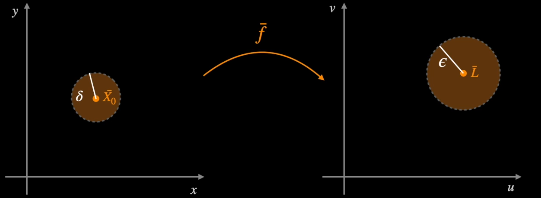
\includegraphics[width=0.7\textwidth]{img/limite.png}
    \label{fig:limite}
\end{figure}

\subsection{Teorema: Unicidad del límite}
Sea $f : \mathbb{R}^n - \{ \vec{X_0} \} \to \mathbb{R}$ (función escalar). Si el límite
$$\lim_{\vec{X} \to \vec{X_0}} f(\vec{X}) = L_1 \text{ y } \lim_{\vec{X} \to \vec{X_0}} f(\vec{X}) = L_2$$
entonces $L_1 = L_2$.

\begin{figure}[H] 
    \centering    
    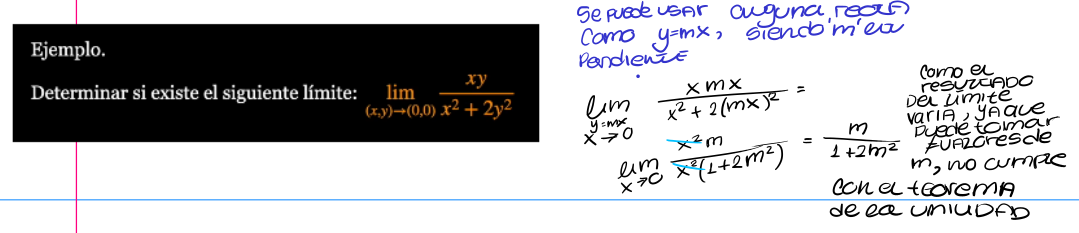
\includegraphics[width=1\textwidth]{img/ej-titulos.png}
    \label{fig:ej-titulos}
\end{figure}

\subsection{Teorema: Infinitesimo por acotado}
Sea $f : \mathbb{R}^n - \{ \vec{X_0} \} \to \mathbb{R}$ (función escalar) una función tal que $\lim_{\vec{X} \to \vec{X_0}} f(\vec{X}) = 0$,
y supongamos que $g : \mathbb{R}^n \to \mathbb{R}$ es una función acotada, esto es, 
existe $M>0$, $|g(\vec{X})| \leq M$ para todo $\vec{X} \in \mathbb{R}^n$. Entonces:
$$\lim_{\vec{X} \to \vec{X_0}} f(\vec{X}) \cdot g(\vec{X}) = 0$$
\begin{figure}[H] 
    \centering    
    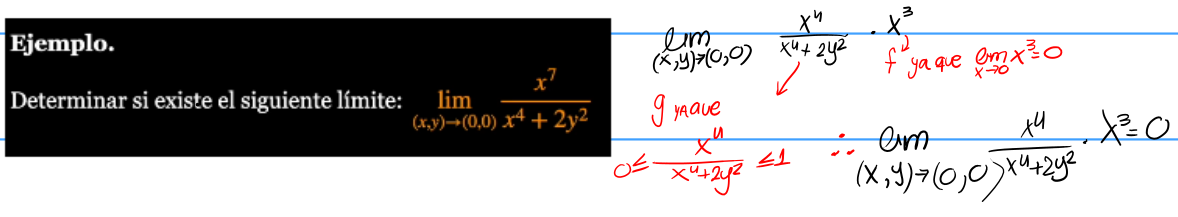
\includegraphics[width=1\textwidth]{img/ej-limites2.png}
    \label{fig:ej-limites2}
\end{figure}